\documentclass[12pt]{article}
\usepackage[utf8]{inputenc} 
\usepackage[ngerman]{babel}
\usepackage{graphicx}
\usepackage{babelbib}
\usepackage{natbib}
\usepackage{url}
\usepackage[german]{algorithm2e}
\usepackage{subcaption}
\usepackage{tikz} 

\begin{document}
\bibliographystyle{mygerapali}
\title{Joggingrouten für Herzpatienten - Mit dynamischer Programmierung passende Laufprofile finden}
\author{Patrick Schulz}

\maketitle

\bigskip
\begin{center} Matrikelnummer: 944808\end{center}

\bigskip
\bigskip
\begin{center} Betreuer: Prof. Dr.-Ing. Jan-Henrik Haunert\end{center}
\begin{center} und Dr. Florian Hillen\end{center}

\bigskip
\bigskip
\bigskip

\begin{figure}[b]
\begin{center} 
\includegraphics[height=120px]{pics/Logo_Osna.jpg} \end{center}
\end{figure}

\pagebreak

\begin{abstract}
Gegeben ist ein zeitabhängiges Leistungsprofil (in kcal/h) und eine festgelegte Wegstrecke. Gesucht wird ein streckenabhängiges Laufprofil (in km/h). Der aus der Wegstrecke und dem Laufprofil entstehende metabolische Energieaufwand soll dem geforderten Leistungsprofil so gut wie möglich entsprechen. Es wird gezeigt, dass dieses Problem anhand von Realinstanzen mit einer Abwandlung des Floyd-Warschall-Algorithmus in annehmbarer Zeit lösbar ist. Die Formel für die Vorhersage des metabolischen Energieaufwands wird von \cite{givoni1971} bereitgestellt. Die benötigten Raumdaten, die für die Berechnung des metabolischen Energieaufwandes benötigt werden, stammen aus frei zugängigen Quellen. Es werden Ansätze angesprochen, um automatisiert Routen zu finden, die für ein gegebenes Leistungsprofil in Frage kämen. Ein Ergebnis von der Eigenimplementierung der erläuterten Algorithmen wird gezeigt und interpretiert. Basierend auf den festgestellten Mängel folgen abschließend Verbesserungsvorschläge für zukünftige Projekte, die es zu behandeln gilt, um das beschriebene Modell für gesundheitliche Anwendungen verwendbar zu machen.
\end{abstract}
\medskip
\noindent 
\\
\textbf{Keywords.} network, graph theory, dynamic programming, metabolic energy

\bigskip

\pagebreak

\tableofcontents

\pagebreak

\section{Einleitung}\label{opening}

Die Gesundheit ist das wichtigste für jeden von uns. Ein glücklicher Mensch ist ein gesunder Mensch. Die Medizin und ihr wissenschaftlicher Kontext plädiert seid Jahrhunderten für eine ausgewogene Ernährung und körperliche Bewegung, um die Gesundheit jedes Individuums zu bewahren. Parallel dazu entstand in den vergangenen Jahrzehnten ein breites Spektrum an Algorithmen für die unterschiedlichsten Routing-Probleme. Insbesondere hat die in 2006 stattgefundene \textit{DIMACS implementation challenge}\footnote{Center for Discrete Mathematics and Theoretical Computer Science - http://www.dis.uniroma1.it/challenge9/index.shtml [Stand März 2016]} den Fortschritt in diesem Themengebiet immens voran gebracht. Alle entwickelten Ansätze zielen darauf ab, den kürzesten Weg zu explizit gewählten Orten möglichst effizient zu finden. Es existiert allerdings kein Ansatz, der ohne Zielknoten auskommt, wenn das Bedürfnis des Menschen nicht darin liegt am schnellsten von einem Ort zum anderen zu gelangen, sondern schlicht sich nur bewegen möchte: \glqq \textit{Der Weg ist das Ziel.}\grqq \footnote{Konfuzius}. \\
Anstelle von Wegpunkten wäre die Anforderung demnach nur eine Routenlänge. Anhand dieser einzigen Angabe soll eine Rundtour erstellt werden. Alternativ wäre auch eine Gesamtzahl der verbrauchten Kalorien als Kriterium für die Routenerstellung denkbar. Der Energieverbrauch lässt sich über die Formel von \cite{givoni1971} abhängig von Körpergewicht, Laufgeschwindigkeit, Streckengradient und Bodenbeschaffenheit gut vorhersagen. Der explizite Energieverbrauch innerhalb der Strecke lässt sich allerdings durch eine einzelne Gesamtangabe nur schwer beeinflussen. Ein konkreter Fall hierfür, wann der genaue Energieverbrauch beeinflussbar sein muss, sind Laufrouten für Herzpatienten. Herzpatienten besitzen idR. ein schwaches Herz, welches trainiert werden muss. Es hätte gesundheitlich fatale Folgen, wenn ein schwaches Herz durch anspruchsvolle Routen überfordert wird und daraufhin versagt. Gleichzeitig soll der Patient aber auch nicht unterfordert werden.\\ 
In den folgenden Kapiteln werden die Anforderungen und Vorstellungen an das gesuchte Laufprofil bei gegeben Leistungsprofil und Wegstrecke konkretisiert und ausformuliert. Desweiteren wird die Berechnung des Energieaufwands mit Hilfe der vorgestellten Energieformel von \cite{givoni1971} umgesetzt. Im darauffolgendem Kapitel wird der Floyd-Warschall-Algorithmus im eigentlichen Sinne vorgestellt, der als Inspiration diente. Anschließend wird beschrieben, wie sich die Idee vom ursprünglichen Algorithmus für das Optimierungsproblem anwenden lässt und zeigen, dass das Optimum in polynomieller Zeit gefunden wird. Danach folgt ein einfacher Ansatz für die Generierung von Rundtouren mit vorgegebener Länge und wie man diesen Ansatz ausbauen kann mit einem Attraktivitätsmaß, sodass die Rundtouren durch attraktive Gegenden verlaufen, wie öffentliche Parks und Wälder. Für die Experimente wird die dafür benötigten Implementationen und Datenquellen angesprochen. Zum Abschluss werden gewählte Ergebnisse von der eigenen Implementation vorgestellt und interpretiert.

\section{Anforderungen}\label{afford}
Gegeben ist eine Laufstrecke $R$. Die Laufstrecke $R$ soll in mehrere, kurze \textit{Etappen} $e_{n} \in R$ aufgeteilt sein. Das in dieser Arbeit behandelte Optimierungsproblem besteht darin für jede Etappe $e_{n}$ eine Laufgeschwindigkeit $v_{n} \in V_{m}$ zu wählen, sodass der errechnete Energieaufwand $g_{n}$ dem Niveau des Leistungsprofils $F$ entspricht. Bemessen soll die Ähnlichkeit der beiden Profile $g_{n}$ und $F$ über die Divergenzkosten $\delta_{n}$. Die Divergenzkosten $\delta_{n}$ sind umso geringer je weniger sich das Energieniveau zwischen den beiden Profilen unterscheidet. \\
Menschen mit Herzproblemen werden womöglich den Großteil des Klientels ausmachen, die davon profitieren würden, wenn es eine Anwendung gäbe, die das besagte Optimierungsproblem behandeln. Basierend auf diesem Aspekt darf dadurch z.B. das erwartete Leistungsprofil $F$ nur zu einem äußerst geringen Grad überschritten werden, um ein schwaches Herz nicht zu überfordern. Die potenziellen Anwender werden somit für den Fortlauf der Ausarbeitung als \textit{Patienten} bezeichnet.\\
Es wird angenommen, dass kein Mensch in der Lage ist eine gezielt vorgegebene Geschwindigkeit zu halten, solange kein Laufband für die Trainingseinheit genutzt wird. Jeder Mensch hat seinen persönlichen Laufrhythmus und seine persönlichen Geschwindigkeitsstufen. Daher müssten Schwankungen im gewünschten Leistungsprofil $F$ berücksichtigt. Die $m$ verschiedenen Laufstufen der Patienten sind dafür in Untersuchungen zu ermitteln und werden in $V_{m}$ festgehalten. Das Leistungsprofil $F$ soll außerdem eine zeitabhängige Funktion sein, weil die Dauer der Lauf-Session von wichtigerer Bedeutung ist als die Distanz, die der Patient laufen soll.\\
\begin{figure}[ht]
	\begin{center}
	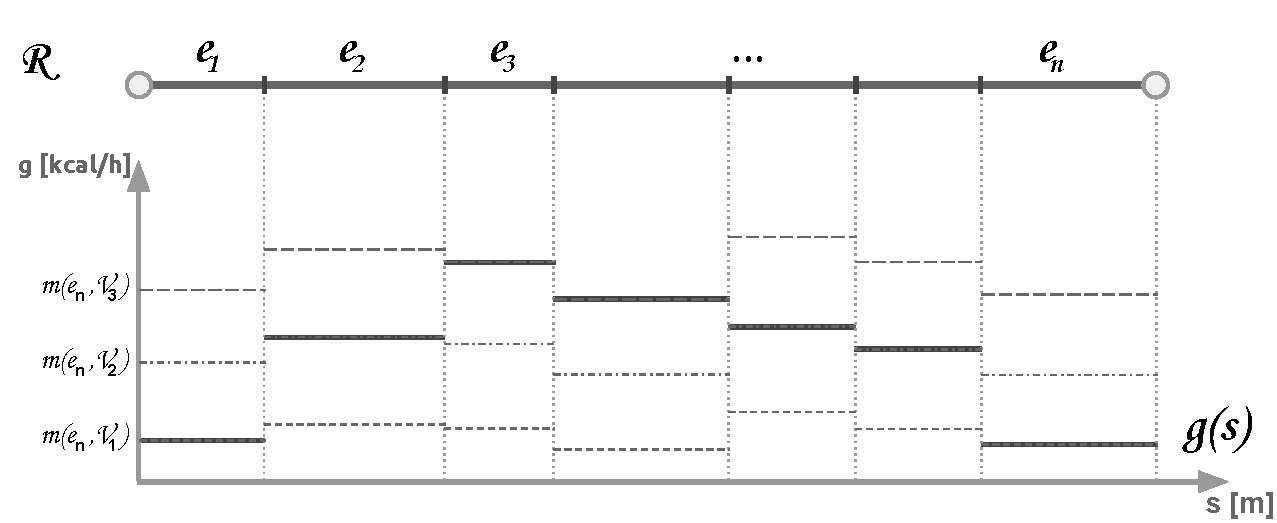
\includegraphics[width=\textwidth]{pics/pdf/001_Power_on_Way.pdf}
	\caption{Abstraktion der Wegstrecke $R$, Visualisierung des Energieverbrauchs $M$ von verschiedenen Laufstufen $V_{m}$ und Etappen $e_n$, und eine mögliches Leistungsprofil g(s) als mögliche Lösung.}
	\label{pic:power_on_way}
	\end{center}
\end{figure}

Die terrestrischen Eigenschaften für jede Etappe $e_{n}$ (konkret: Gradient $G_{n}$, Streckenlänge $l_{n}$, und Bodenbeschaffenheit $\eta_{n}$) sollen für das Modell des Optimierungsproblems bereits gestellt sein. Innerhalb einer Etappe $e_{n}$ sollten die terrestrischen Eigenschaften konstant sein, sodass der Energieaufwand pro Etappe für eine vorgegebene Laufgeschwindigkeit $v_{n}$ ebenfalls konstant bleibt. Über die Quellen und Aufbereitung der bereitgestellten, terrestrischen Eigenschaften für die Experimente wird in den späteren Abschnitten \ref{routing} und \ref{experiment} eingegangen.\\
Aus den gewählten Laufgeschwindigkeiten $v_{n}$ für jede Etappe $e_{n}$ lässt sich das strecken-abhängige, ermittelte Leistungsprofil $g(s)$ ableiten (siehe Abbildung \ref{pic:power_on_way}). Aus dem gewünschtem Leistungsprofil $F$ entsteht eine zeitabhängige, diskrete und in Intervallen unterteilte Funktion $f(t)$. Eine strecken-abhängige Funktion $f(s)$ würde den Vergleich mit $r(s)$ und somit die Möglichkeit der Berechnung von $\delta_{n}$ zwar vereinfachen, aber nicht den oben genannten Anforderungen entsprechen.\\
Es besteht eine hohe Wahrscheinlichkeit, dass eine vorgegebene Laufstrecke $R$ länger ist, als es von dem eigentlichen Leistungsprofil $F$ benötigt wird. Daran scheitert jedoch das Lösen des Optimierungsproblems nicht zwangsläufig. Die restliche Strecke soll dann als \textit{Auslauf-} und \textit{Ruhestrecke} $F_{B}$ behandelt werden (siehe Abbildung \ref{pic:power_on_time}). Die Divergenzkosten $\delta_{n}$ vom $F_{B}$ Segment sollen weniger gewichtet werden als vom Leistungsprofil $F$. Das $F_B$ Segment muss nicht vom gemessenen Leistungsprofil $g(s)$ gedeckt werden. Wenn eine Wegstrecke $R$ zu kurz ist und somit das Leistungsprofil $F$ nicht vollständig abdecken kann, dann können keine gültigen Lösungen für das Optimierungsproblem gefunden werden.

\begin{figure}[ht]
	\begin{center}
	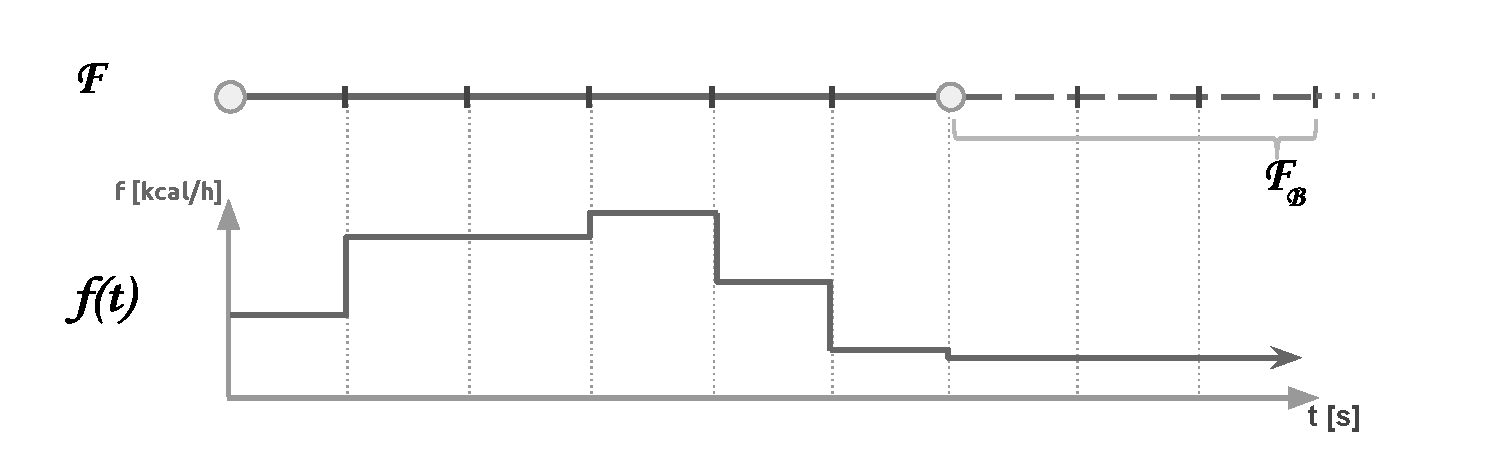
\includegraphics[width=\textwidth]{pics/pdf/002_Power_on_Time.pdf}
	\caption{Abstraktion des Leistungsprofils $F$, dem Auslaufsegment $F_{B}$ und deren Vereinigung in $f(t)$.}
	\label{pic:power_on_time}
	\end{center}
\end{figure}

\paragraph{Energieformel} Die \textit{Energieformel} zur Berechnung des metabolischen Energieaufwandes ist das Ergebnis einer Untersuchungsreihe von \cite{givoni1971}. Es wurden mehrere Probanden untersucht, die auf Laufbändern Distanzen mit unterschiedlichen Steigungen und Geschwindigkeiten liefen. Die Formel, die sich aus der Regression der verschiedenen Messungen ergab, lautet wie folgt:
\begin{equation}
	M = \eta * W \left[ 2.3 + 0.32 \left( V - 2.5 \right)^{1.65} + G \left( 0.2 + 0.07 \left( V - 2.5 \right) \right) \right] 
\end{equation}
Die Variablen haben die folgende Bedeutung:
\begin{itemize}
\item[$M$] der ermittelte Energieverbrauch in Kilokalorien pro Stunde
\item[$\eta$] ein Koeffizient, der die Bodenbeschaffenheit repräsentiert.
\item[$W$] das Gewicht des Läufers inklusive Gepäck und Anzug in Kilogramm.
\item[$V$] die Laufgeschwindigkeit in Kilometer pro Stunde 
\item[$G$] der Gradient des Wegstrecke in Prozent
\end{itemize}
Für den $\eta$-Koeffizienten stellen die Autoren wenige Beispiele: $\eta = 1.0$ entspricht der \textit{perfekten} Bodeneigenschaft eines Laufbandes, $\eta = 1.2$ eine befestigte Straße und $\eta = 1.8$ für sehr nachgiebigen Boden, wie eine Sanddüne. Für weitere Differenzierung befindet sich in Abschnitt \ref{experiment} eine Tabelle mit verschiedenen Bodentypen und $\eta$-Werte, die für die Experimente verwendet wurden. In der Tabelle \ref{tab:m_example} sind ein paar Beispiele als Referenz für die erwartenden Energiewerte aufgeführt. Die Energieformel ist nicht dafür ausgelegt für starke Gefälle kleiner -5 Prozent nachvollziehbare Werte zu finden. Es existieren noch weitere Einschränkungen für die Formel, wie z.B. die Annahme, dass externes Gewicht möglichst am Masseschwerpunkt des Patienten gelegen ist. Aktuellere Beiträge aus der Physiologie stellen präzisere Formeln auf, die unter Anderem auch die Schrittweite, Lauftypus und die genaue Gewichtsverlagerung des Patienten mit einbeziehen - der Gradient wird in den moderneren Formeln allerdings nicht mit berücksichtigt, welcher für die geoinformationstechnische Motivation interessant ist. Eine Übersicht über die in der Physiologie bekannten Energieformeln werden von \cite{hall2004} vorgestellt. Für die Experimente des Optimierungsproblems genügt die relativ einfache Energieformel von \cite{givoni1971}. Wenn es darum ginge genauere und zuverlässigere Modelle für den Energieverbrauch zu entwickeln, um daraus eine plausible Anwendungen erstellen zu können, sollten zur Optimierung Ansätze, wie die von \cite{pandolf1976} und \cite{sun2013} mit in Betracht gezogen werden. 
\begin{table}
\begin{tabular}{c|c|c|c||r}
	Geschwindigkeit $V$&Steigung $G$&Gewicht $W$&Terrain $\eta$&Verbrauch $M$\\ \hline \hline
	5.0&0.0&80.0&1.2&360.12\\
	5.0&5.0&80.0&1.2&540.12\\
	5.0&-2.5&80.0&1.2&270.12\\
	10.0&0.0&80.0&1.2&1074.43\\
	10.0&5.0&80.0&1.2&1422.43\\
	10.0&-2.5&80.0&1.2&900.43\\
\end{tabular}
\caption{Verschiedene errechnete Energiewerte in [kcal/h] mit den gegebenen Werten. Veränderungen von $G$ und $W$ skalieren mit dem Energieverbrauch $M$ linear.}
\label{tab:m_example}
\end{table}

\section{Das Optimierungsproblem lösen}\label{optimize}
Die Idee wie man das Optimierungsproblem optimal lösen kann und eine Möglichkeit findet die Leistungsprofile $g(s)$ und $f(t)$ mit den unterschiedlichen variablen Abhängigkeiten abzugleichen, basiert auf der algorithmischen Idee von \cite{floyd1962} und \cite{warshall1962}. Im folgenden Abschnitt \ref{Floyd} wird der ursprüngliche Algorithmus vorgestellt und dessen Möglichkeiten der Erweiterbarkeit gezeigt. In dem darauffolgenden Abschnitt \ref{apply} wird die Idee vom ursprünglichen Algorithmus für das Optimierungsproblem der Leistungsprofile angepasst.
\subsection{Algorithmus von Floyd und \cite{warshall1962}}\label{Floyd}
Der All-Pair-Shortest-Path-Algorithmus von Floyd und Warshall ist ein vorbildliches Beispiel für dynamische Programmierung. Eine Charakteristik von Problemen, die durch dynamische Programmierung gelöst werden können, ist die Tatsache, dass das Hauptproblem aus mehreren, gleichartigen Teilproblemen zerlegt werden kann. Das Lösen der Teilprobleme und das Wiederverwenden der Teillösungen führen im Endeffekt zur Lösung des eigentlichen Problems \citep{bellman1957}.\\
Gegeben sei ein kanten-gewichteter, gerichteter Graph $G = (V,E)$. Die Kosten der Kanten $E$  dürfen negativ sein, allerdings darf kein Kreis in $G$ existieren, der beim Durchlaufen negative Kosten verursacht. Ein solcher Kreis, wenn man ihn oft genug durchläuft, wäre in der Lage für jedes Knotenpaar$(u,v)$ im Graphen $G$ eine Route $R(u,v)$ zu finden, die immer günstiger ist als die bestehende, bekannte, kosten-geringste Route. Die nächst-kosten-geringere Route würde dann immer einen Durchlauf mehr durch den negativen Kreis verlaufen als die bisherige Route. Über drei ineinander verschachtelte Schleifen wird eine Tabelle befüllt, die alle kürzesten Pfade zwischen beliebigen Knotenpaaren $(u,v)$ speichert und bestehende Lösungen als Teillösungen verwendet.

\begin{algorithm}
\KwData{Kostenmatrix $w$ von $G$}
\For{$i \in E$}{
	\For{$j \in E$}{
		d[i,j] = w[i,j]\;
	}
}
\For{$k \in E$}{
	\For{$i \in E \setminus k$}{
		\For{$j \in E \setminus k$}{
			d[i,j] = min(d[i,j], d[i,k] + d[k,j])\;
		}	
	}
}
\caption{All-Pair-Shortest-Path-Algorithmus von \cite{floyd1962}}
\label{alg:floyd}
\end{algorithm}

Der Algorithmus nutzt die folgende Beobachtung: Wenn ein schnellster Weg zwischen dem Knotenpaar $(i,j)$ durch $k$ verläuft, dann sind die berechneten Teillösungen von $(i,k)$ und $(k,j)$ bereits optimal. Daher prüft der Algorithmus über alle Knotenpaare, ob die Summe der Teillösungen von $(i,k)$ und $(k,j)$ kleiner sind als die bestehende bekannte Lösung von $(i,j)$.\\

\begin{algorithm}
\KwData{Kostenmatrix $w$ von $G$}
\For{$i \in E$}{
	\For{$j \in E$}{
		\If{w[i,j] = 1}{d[i,j] = 1\;}
	}
}
\For{$k \in E$}{
	\For{$i \in E \setminus k$}{
		\For{$j \in E \setminus k$}{
			\If{d[i,k] = 1 {\bf and} d[k,j] = 1}{d[i,j] = 1\;}
		}	
	}
}
\caption{Erreichbarkeits-Algorithmus von \cite{warshall1962}}
\label{alg:warshall}
\end{algorithm}

\pagebreak
Der Algorithmus \ref{alg:warshall} von \cite{warshall1962} ist vom Grundaufbau identisch wie der Algorithmus \ref{alg:floyd} von \cite{floyd1962}. Beide Algorithmen besitzen durch die dreifach-verschachtelte Schleife über alle Knoten $V$ im Graphen $G$ eine Laufzeit von $O(V^3)$. Die Schleife über alle Knotenpaare wird programmiertechnisch mit einer doppelt verschachtelten Schleife realisiert. Der Unterschied besteht in der Zielsetzung: Die Algorithmen unterscheiden sich im Informationsgehalt und füllen die Tabellen mit unterschiedlichen Daten. Algorithmus \ref{alg:floyd} produziert eine Distanzmatrix des Graphen $G$ und Algorithmus \ref{alg:warshall} produziert eine Erreichbarkeitstablle vom Graphen $G$; Wenn ein Knotenpaar $(i,j)$ im Graphen erreichbar ist, dann soll die Verbindung in der Tabelle mit einer $1$ markiert sein. 

Im Algorithmus \ref{alg:warshall} wird dann die Regel genutzt, dass wenn ein Knoten $j$ von Knoten $k$ und Knoten $k$ von Knoten $i$ aus erreichbar ist, dann ist Knoten $j$ auch von Knoten $i$ über $k$ aus erreichbar: 
\begin{equation}
	d[i,k] = 1 \& d[k,j] = 1 \rightarrow d[i,j] = 1
	\label{eq:erreichbarkeit}
\end{equation}
Als Ergebnis für den Graphen in der Abbildung \ref{pic:floyd_graph} entsteht nach dem Algorithmus \ref{alg:warshall} eine Tabelle, in der jede Zelle eine $1$ eingetragen ist, weil jeder Knoten von jedem anderen Knoten im Graphen aus erreichbar ist.

\begin{figure}[ht]
	\begin{center}
	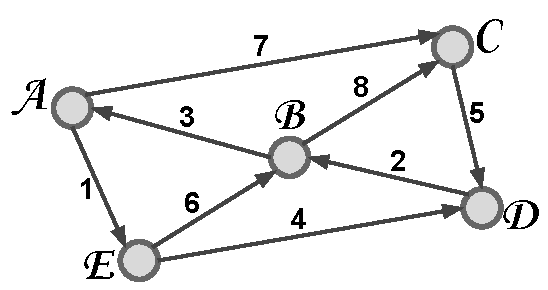
\includegraphics[width=160pt]{pics/pdf/003_Floyd_Graph.pdf}
	\caption{Beispielgraph mit Knotenbezeichnung und Kantengewichten}
	\label{pic:floyd_graph}
	\end{center}
\end{figure}

Für den Graphen in Abbildung \ref{pic:floyd_graph} folgt nun ein Beispiel, wie eine Distanztabelle für den Graphen mit dem Algorithmus \ref{alg:floyd} entsteht. Gegeben ist uns die \textit{Tabelle \ref{tab:floyd_start} links}, die alle Kosten zwischen allen Knotenpaaren beinhaltet, die auch über eine direkte Kante verbunden sind. In der ersten $k$-Iteration mit $k = A$ stellt sich heraus, dass die Knotenpaare $(B,C)$ und $(B,E)$ über $A$ Verlaufen. Der bisherige Distanzwert von Knoten $B$ zu $E$ beträgt \textit{8} - laut \textit{Tabelle \ref{tab:floyd_start} links}. Die Summe der Strecke $(B,C)$ über $A$ beträgt $d[B,A] + d[A,C] = 3 + 7 = 10$. Die Strecke $(B,C)$ über $A$ ist nicht kürzer als die bisher bekannte kürzeste Strecke; Es werden somit keine Einträge in der Distanztabelle aktualisiert. Eine Strecke von Knoten $B$ zu $E$ ist vor der ersten k-Iteration nicht bekannt gewesen (und mit $ $ markiert). Die Teilstrecken $(B,A)$ und $(A,E)$ sind bekannt, somit gibt es auch eine Strecke $(B,E)$ über $A$ mit den Kosten $d[B,A] + d[A,E] = 3 + 1 = 4$. Die Distanztabelle wird in der Zelle $B,E$ mit $4$ aktualisiert. Für die restlichen Knotenpaare fehlen von Knoten $A$ aus die benötigten Teilstrecken bzw. die Teilstrecken sind noch nicht bekannt, welches in der Teilstreckensumme immer $\infty$ ergibt und definitiv nie kleiner sein wird als die bisher bekannten Strecken. Die erste $k$-Iteration mit $k = A$ ist an dieser Stelle dann beendet.

\begin{table}
\begin{tabular}{r||c|c|c|c|c}
	Knoten&A&B&C&D&E\\ \hline \hline
	A&0&$\infty$&6&$\infty$&1\\
	B&3&0&8&$\infty$&$\infty$\\
	C&$\infty$&$\infty$&0&5&$\infty$\\
	D&$\infty$&2&$\infty$&0&$\infty$\\
	E&$\infty$&7&$\infty$&4&0\\
\end{tabular}
\hspace*{20pt}
\begin{tabular}{r||c|c|c|c|c}
	Knoten&A&B&C&D&E\\ \hline \hline
	A&0&7&6&5&1\\
	B&3&0&8&8&4\\
	C&10&7&0&5&11\\
	D&5&2&10&0&6\\
	E&9&6&14&4&0\\
\end{tabular}
\caption{Distanztabellen zu den verschiedenen Zuständen im Diagramm: \textbf{Links} Startzustand mit den Kosten der direkten Kantenverbindungen $E$. \textbf{Rechts} Endergebnis nach n = 5 k-Iterationen.}
\label{tab:floyd_start}
\end{table}

Während der zweiten $k$-Iteration mit $k = B$ entstehen 5 Aktualisierungen in der Distanztabelle. Die Werte werden nach dem selben Schema erfasst, wie auch zuvor in der erste $k$-Iteration. Interessant hier ist die Strecke $(D,E)$, die aus der Wegstrecke $(D,B)$ und $(B,E)$ entsteht. Die Kosten belaufen sich auf $d[D,B] + d[B,E] = 2 + 4 = 6$. Es fällt auf, dass die Kosten der Strecke $(B,E)$ in der vorherigen k-Iteration berechnet wurde und in dieser Iteration als Teillösung wiederverwendet werden. In der \textit{Tabelle \ref{tab:floyd_zwischen} links} ist die Distanztabelle abgebildet, wie sie nach der zweiten k-Iteration aussieht. Nach allen Iteration sieht die Distanztabelle so aus, wie in \textit{Tabelle \ref{tab:floyd_start} rechts} angegeben. \textit{Tabelle \ref{tab:floyd_zwischen} rechts} zeigt nochmal zusätzlich den Zustand der  Ausgangstabelle nach der vierten $k$-Iteration. 
\begin{table}
\begin{tabular}{r||c|c|c|c|c}
	Knoten&A&B&C&D&E\\ \hline \hline
	A&0&$\infty$&6&$\infty$&1\\
	B&3&0&8&$\infty$&4\\
	C&$\infty$&$\infty$&0&5&$\infty$\\
	D&5&2&10&0&6\\
	E&10&7&15&4&0\\
\end{tabular}
\hspace*{20pt}
\begin{tabular}{r||c|c|c|c|c}
	Knoten&A&B&C&D&E\\ \hline \hline
	A&0&13&6&11&1\\
	B&3&0&8&13&4\\
	C&10&7&0&5&11\\
	D&5&2&10&0&6\\
	E&9&6&14&4&0\\
\end{tabular}
\caption{Distanztabellen zu den verschiedenen Zuständen im Diagramm: \textbf{Links} Zwischenergebnis nach der zweiten k-Iteration (k = \textit{B}).\\ \textbf{Rechts} Zwischenergebnis nach der vierten k-Iteration (k = \textit{D}).}
\label{tab:floyd_zwischen}
\end{table}

Wenn man bei beiden Algorithmen eine Zusatzinformation abspeichert über welchen Knoten $k$ die neue kürzeste Strecke $(i,j)$ verläuft, dann lässt sich später für die Weiterverarbeitung neben der Distanz auch der genaue Streckenverlauf rekursiv ermitteln.

\subsection{Single Source Shortest Path-Variation}\label{sssp_chapter}

Mit dem Ansatz aus den Algorithmen von Floyd und Warshall kann man nicht nur All-Pair-Shortest-Path und Erreichbarkeits-Probleme lösen. Der Ansatz lässt sich auch für Single-Source-Shortest-Path (kurz \textit{SSSP}) Probleme anwenden mit der Besonderheit, dass verschiedene Touren für ein Knotenpaar berechnet werden mit unterschiedlichen Kosten. Voraussetzung besteht darin, dass die Kosten  positiv, sowie ganzzahlig sind ($w \in N$) und eine annehmbare Obergrenze $W_{max}$ für die Kostensumme gebildet werden kann. Basierend darauf lässt sich für einen gewählten Startpunkt $S$ folgender Algorithmus \ref{alg:sssp_simple} formulieren:

\begin{algorithm}
\KwData{Kostenmatrix $w$ von $G$}
\textit{ascend}[$S$, 0] = $S$ \;
\For{$c \rightarrow 0 .. W_{max}$}{
	\For{$j \in E$}{
		\For{$i \in E$}{
			\If{\textit{ascend}[j,(c - w[i,j])] != $\infty$ }{\textit{ascend}[j,c] = j\; break\;}
		}	
	}
}
\caption{Single-Source-Shortest-Path-Algorithmus für Strecken mit unterschiedlichen Kosten. (Laufzeit \textit{O($V^2*Z_c$)}}
\label{alg:sssp_simple}
\end{algorithm}

Der Algorithmus iteriert aufsteigend über alle möglichen Kostensummen $c$ und überprüft, ob jeweils ein Knoten $j$ vom Startknoten $S$ aus mit den Kosten $c$ erreichbar ist. Ermittelt wird die Erreichbarkeit über die bestehenden, eingehenden Kanten. Wenn ein Knoten $i$ zuvor mit den Kosten $c - w[i,j]$ erreichbar war, dann ist $j$ auch mit den Kosten $c$ über den Knoten $i$ erreichbar. Für den Graphen in Abbildung \ref{pic:azyk_graph} folgt nun die Tabelle \ref{tab:sssp_result} mit den Ergebnissen von Algorithmus \ref{alg:sssp_simple} bis $c = 16$.  Die Ergebnis-Tabelle ist bei einem azyklischen Graphen weniger gefüllt, als bei einem zyklischen oder ungerichteten Graphen, indem die Möglichkeit besteht, dass Routen zwischen zwei Knoten alternieren können.

\begin{table}
\begin{tabular}{c|r|r|r|r|r|r|r|r|r|r|r|r|r|r|r|r}
c&0&1&2&3&4&5&6&7&8&9&10&11&12&13&14&15\\ \hline
A&0& & & & & & & & & & & & & & &\\
B& &A& & & & & & & & & & & & & &\\
C& & & & &B&A& & & & & & & & & &\\
D& & & & & & & &B&C&C& & & & & &\\
E& & & & & & & & & &D&D&D& & & &\\
F& & & & & & & & & & & & &C&C&E&E\\
G& & & & & & & & & & & & & &F&F&F\\
H& & & & & & & & & & & & & & & &G\\
\end{tabular}
\caption{\textit{ascend}-Ergebnis des Single-Source-Shortest-Algorithmus \ref{alg:sssp_simple} für den gerichteten Graph in Abbildung \ref{pic:azyk_graph} }
\label{tab:sssp_result}
\end{table}

Falls es mehrere Möglichkeiten gibt einen bestimmten Knoten $j$ mit den Kosten $c$ zu erreichen, wird mit dem Algorithmus \ref{alg:sssp_simple} bisher immer die zuerst gefundene Lösung gewählt. Dieses Verhalten lässt sich erweitern, indem man z.B. zwei Kostentypen $w_{1}$ und $w_{2}$ einführt. Die Kosten $w_{1}$ entsprechen den ganzzahligen Kosten $w$ aus Algorithmus \ref{alg:sssp_simple}. Nach den Kosten $w_{2}$ wird entschieden, welche Option $i$ für die Erreichbarkeit von $j$ gewählt werden soll. Diese Idee der zwei Kostentypen wird für das Optimierungsproblem im nächsten Abschnitt \ref{apply} angewendet.

\begin{figure}[ht]
	\begin{center}
	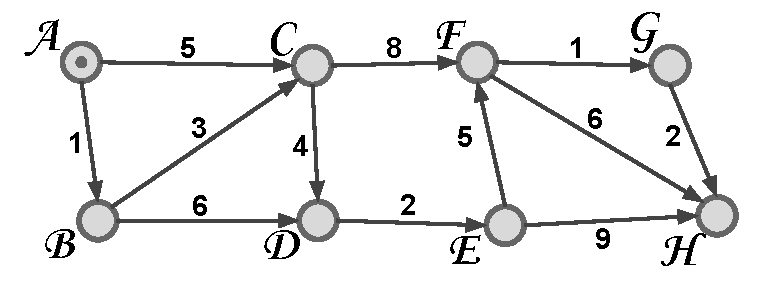
\includegraphics[width=280pt]{pics/pdf/004_Azyklischer_Graph.pdf}
	\caption{Beispielhafter, azyklischer Graph mit Knotenbezeichnung und Kantengewichten}
	\label{pic:azyk_graph}
	\end{center}
\end{figure}
\pagebreak

\subsection{Anwendung}\label{apply}
Die Möglichkeit zum Abgleich mit dem zeitabhängigen Leistungsprofil $f(t)$ für jede Etappe $e_{n}$ muss gewährleistet werden, um die Divergenzkosten $\delta_{n}$ berechnen zu können. Angenommen der Zeitpunkt $a_{n}$ wäre bekannt, wann man sich an einem bestimmten Meilenstein $v_{n}$ der Strecke befindet, sowie die Zeitspanne $b_{n,m}$, die man für eine Etappe $e_{n}$ benötigt bei einer vorgegeben Laufgeschwindigkeit $V_{m}$. Dann wäre man für diesen Zeitpunkt $a$ und Zeitspanne $b$ in der Lage aus $f_{t}$ einen Leistungswert zu ermitteln, der für den gewählten Intervall $ I = \left[ a_{n} : a_{n}+b_{n,m}\right]$ gelten soll. Die Abbildung \ref{pic:get_power} zeigt zwei verschiedene Möglichkeiten, wie man den gewünschten Energiewert aus dem Leistungsprofil $f(t)$ für einen gewählten Interval $I$ ermitteln kann. Die links dargestellte Methodik ermittelt den Modalwert, die rechte Methodik errechnet den Durchschnittswert im Interval $I$. Beide Methoden verfälschen zu einem gewissen Grad den Ursprungswert, wenn Interval $I$ sich über mehrere, verschiedene Energieniveaus von $f(t)$ erstreckt. Der Modalwert behält im Gegensatz zum Durchschnittswert die definierten Leistungstufen in $F$ und \textit{interpoliert} keine neuen Stufen. Um der Verfälschung generell entgegenzuwirken, sollten bei der Umsetzung die einzelnen Etappen der Wegstrecke $R$ möglichst kurz gehalten werden oder die Zeitintervalle der Energieniveaus von $F$ möglichst groß sein. In Abschnitt \ref{experiment} folgt hierzu noch eine Ergänzung, was das richtige Verhältnis betrifft.

\begin{figure}[ht]
	\begin{center}
	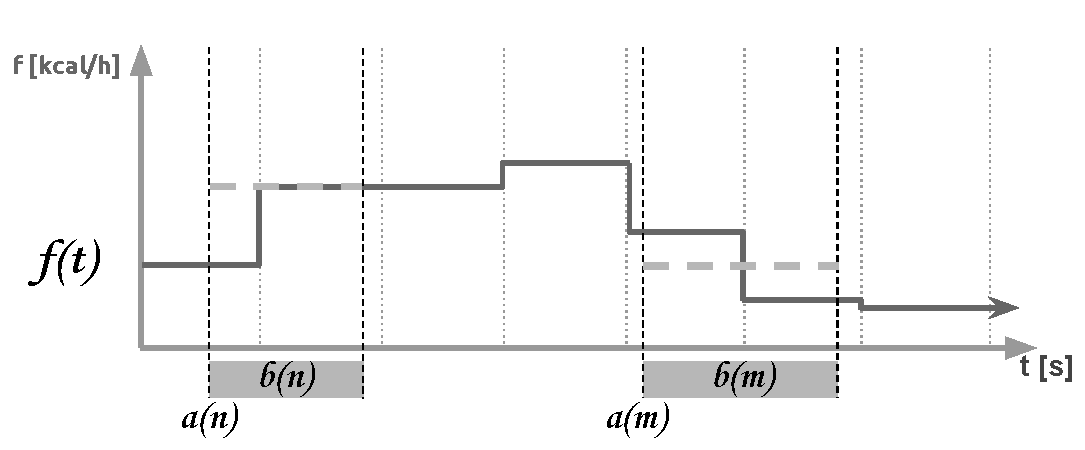
\includegraphics[width=360pt]{pics/pdf/007_get_proposed_Power.pdf}
	\caption{Zwei Varianten zur Ermittlung des Energieniveaus via Zeitpunkt $a(n)$ und Zeitspanne $b(n,m)$. \textit{Links}: Modalwert, \textit{Rechts}: Durchschnitt}
	\label{pic:get_power}
	\end{center}
\end{figure}

Wenn die oben erwähnte Methodik zur Ermittlung des Energieniveaus zufriedenstellend ist, dann kann der Algorithmus \ref{alg:sssp_simple} aus Kapitel \ref{sssp_chapter} für die Zwecke des Optimierungsproblems angepasst werden (siehe Algorithmus \ref{alg:sssp_optimized}):

\begin{algorithm}[ht]
\KwData{Etappenlänge $l$ von $e \in R$}
w[$S$,0] = 0;
v[$S$,0] = 0;
\For{$e \in R$}{
	\For{$m \in V_m$}{
		d[e,m] = \textit{round}($l[e] / m * 3.6$)\;
		g[e,m] = \textit{givoni}(e,m)\;
		\For{$t \rightarrow 0 .. t_{max}$}{
			$\delta$[e,m,t] = $( g[e,m] - f(c, d[e,m])^2$			
		}
	}	
}
\For{$t \rightarrow 0 .. t_{max}$}{
	\For{$e \in R$}{
		\For{$m \in V_{m}$}{
			current = w[e-1, t-d[e-1,m]] + $\delta$[e,m,t]\; 
			\If{current < w[e,t]}{
				w[e,t] = current\;
				v[e,t] = m;
			}
		}
	}
}
\caption{Single-Source-Shortest-Path-Algorithmus (kurz: \textit{SSSP}) für das Optimierungsproblem. (Laufzeit \textit{O($V*V_m*Z_c$)}}
\label{alg:sssp_optimized}
\end{algorithm}

Gegeben sind uns die Streckenlängen $l$ aller Etappen $e_n$ von der Wegstrecke $R$. Im ersten Schritt werden alle Zeiten $d$ berechnet, die man für jede Etappe $e_{n}$ mit der vorgegebenen Laufgeschwindigkeit $V_m$ benötigen würde. Die Zeiten sind auf ganze Sekunden aufgerundet, damit diese die Anforderungen für den Kostentypus $w_1$ vom SSSP-Algorithmus aus Kapitel \ref{alg:sssp_simple} entspricht. Als Nächstes wird der Energieverbrauch $g$ für jede Etappe $e_{n}$ mit der vorgegebenen Laufgeschwindigkeit $V_m$ berechnet. Sowohl $d$, als auch $g$ werden anschließend benötigt, um für jeden Zeitpunkt $c$ bis $t_max$ die Divergenzkosten $\delta$ für jede Kombination von $e_n$ und $V_m$ zu berechnen. Dabei spannen Zeitpunkt $c$ und Dauer $d$ den Intervall auf, um den gewünschten Energiewert von $f(t)$ zu ermitteln, wie zuvor in Abbildung \ref{pic:get_power} dargestellt. Die Differenz zum errechneten Energiewert $g$ zu dem gewünschten Energiewert $f$ wird quadriert und als Divergenzkosten $\delta$ gespeichert. Die Quadrierung hat den Effekt, dass größere Differenzen stärker \textit{bestraft} werden als kleinere Abweichungen. Die $\delta$-Werte entsprechen dem Kostentypus $w_2$, nachdem entschieden werden soll, welche Option der Erreichbarkeit bevorzugt werden soll. Sowohl $w_1$ als auch $w_2$ (alias. $d$ und $\delta$) stehen für den eigentlichen SSSP-Algorithmus zur Verfügung. \\
Beginnend mit dem Zeitpunkt c = 0 werden zwei Tabellen $w$ und $v$ befüllt, die jeweils die bisherigen Kosten $w_2$ für die Teilstrecke von $S$ bis $v_n$ abspeichert und die gewählte Laufgeschwindigkeit $V_m$ für die zuvor gelaufene Etappe $e_n$ festhält. Der Vorgängerknoten von einem Meilenstein $v_n$ ist, wie in Abbildung \ref{pic:graph_simple} dargestellt, im Graphen von $R$ immer bekannt, weil es sich um eine azyklische Kette handelt. Von einem Meilenstein zum nächsten gibt es mehrere Kanten, welche die unterschiedlichen Laufgeschwindigkeitsstufen $V_m$ repräsentieren mit deren eigenen Streckendauern $d$. Deshalb wird anstatt des Knotenvorgängers die verwendete Kante in $v$ gespeichert. Eine komplexere Variante sich den Graphen vorzustellen, wird am Ende der Ausarbeitung in der Abbildung \ref{pic:graph_right} gezeigt in der eigentliche Graph dupliziert wird für jeden Zeitpunkt und die ausgehenden Kanten eines Meilensteins sich zu dem selben Meilenstein an verschiedenen Zeitpunkten führen. Die Kanten besitzen den Kostentypus $w_2$. Würde man den azyklischen Graphen in Abbildung \ref{pic:graph_simple} ausbauen wie in Abbildung \ref{pic:graph_right}, dann könnte man darauf den ursprünglichen SSSP-Algorithmus von Kapitel \ref{optimize} anwenden.\\ 
Aufgrund der großen Vorarbeit der benötigten Daten ist der Algorithmus \ref{alg:sssp_optimized} nicht für umfangreiche Graphen, wie zum Beispiel Straßennetze gedacht. Für größere Straßennetzemüssten für die Vorprozessierung noch Optimierungen gefunden werden. Um den Vorprozessierungsaufand zu mindern, ist die bisherige Vorangehensweise die passende Wegstrecke $R$ aus dem Graphen $G$ zu finden. Im nächsten Abschnitt wird nun die Erstellung des \textit{Sub-Graphen} $R$ vorgestellt. 
 
\begin{figure}[h]
	\begin{center}
	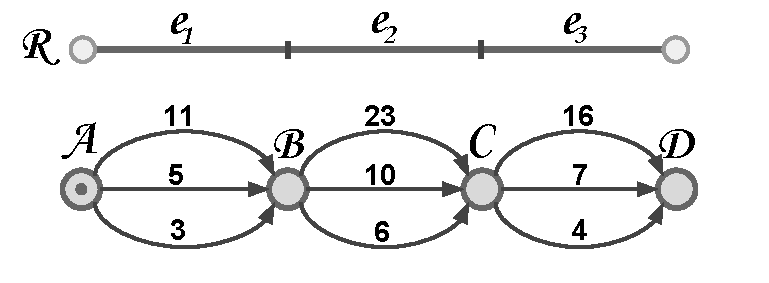
\includegraphics[width=320pt]{pics/pdf/005_Graph_der_Optimierung_Falsch.pdf}
	\caption{Einfache Graphvorstellung für das Optimierungsproblem auf dem Wegstrecke $R$. Die abgebildeten Kantenkosten $w_1$ entsprechen der Dauer $d$ in Sekunden.}
	\label{pic:graph_simple}
	\end{center}
\end{figure}

\section{Das Routenfindungsproblem}\label{routing}
Wie bereits in der Einleitung (Abschnitt \ref{opening}) angesprochen, gibt es keinen Graphen-Algorithmus, der für die vorgestellten Anforderungen erstellt wurde. Die erstellte Rundtour muss nur die Eigenschaft einer expliziten Länge $l$ aufweisen. Bis auf einen Startknoten werden keine weiteren Zwischenpunkte angegeben. Für die Experimente in Abschnitt \ref{experiment} wird nun ein relativ einfaches Verfahren vorgestellt, wie über 3 Stützpunkte $v_{a}, v_{b}, v_{c} \in V$ (inklusive Startknoten) eine Rundtour der Länge $l$ generiert werden kann.\\
Gegeben ist ein kanten-gewichteter, ungerichteter Graph $G = (V,E)$ im zweidimensionalen Raum, ein Startknoten $S \in V$ und ein Zielwert $l_{R}$. Der erste Stützpunkt $v_a$ entspricht dem Startknoten $S$. Stützknoten $v_{b}$ ist ein zufälliger Knoten des Graphen, der maximal $l_{R}/2$ von $v_a$ entfernt liegt. Die Strecke zwischen $v_{a}$ und $v_b$ wird in $l_{ab}$ erfasst. Für den letzten Stützpunkt $v_{C}$ werden jeweils von $v_{a}$ und $v_{b}$ kürzeste Wegebäume zu allen Knoten im Umkreis von $l_{bca} = l_{R} - l_{ab}$ der jeweiligen Baumwurzel berechnet. Die abgescannten Knoten der beiden Suchbäume werden miteinander abgeglichen. Ermittelt wird für jeden Knoten $n$ die Länge $l_{bna} = l_{bn} + L_{na}$ über die Summe der Distanzen zu $v_{a}$ und $v_{b}$. Aus der Menge der abgescannten Knoten $V_{n}$ soll der Knoten ausgewählt werden, bei dem $|l_{bna} - l_{bca}|$ minimal ist.\\
Der beschriebene Ansatz ist rudimentär und ausbaufähig. Es wird nicht gewährleistet, dass die \textit{Qualität} der Stützpunkte für die Rundtour $R$ sinnvoll ist. Die Knoten können zum Beispiel in eine Sackgasse verlaufen oder in ein für Jogger weniger attraktives Gebiet führen. Auch zwischen den Stützpunkten wird nicht unbedingt die attraktivste, sondern nur die kürzeste Strecke gewählt. Um die \textit{Qualität} der generierten Routen zu verbessern, ist für die Experimente ein \textbf{Attraktivitätsmaß $J(e); e \in E$} eingeführt, welches sich aus GPS-Trajektorien von bestehenden, bekannten Joggingrouten ableiten lässt. Die GPS-Trajektorien lassen sich mit dem bestehenden Straßennetz abgleichen - je mehr Trajektorien von verschiedenen Joggingrouten auf eine Kante gematcht werden, desto attraktiver ist der betroffene Weg, der durch die Kante repräsentiert wird. Das Attraktivitätsmaß kann daraufhin an zwei Stellen für das bestehenden Routengenererierungs-Verfahren verwendet werden: Bei der Wahl des zufälligen Stützknotens $v_{b}$ kommt ein weiteres Kriterium hinzu, dass mindestens eine der inzidenten Kanten von $v_{b}$ ein bestimmtes Minimum an Attraktivität besitzen soll. Für die kürzesten Wege lässt sich außerdem eine Kostenfunktion  beschreiben, die die \textit{gefühlte} Länge eines Weges widerspiegeln soll. Je attraktiver die Strecke, desto günstiger die Kosten, desto eher wird die betroffene Kante für die kürzeste Wege mit den neuen Kosten verwendet. Unter Berücksichtigung dieser Kriterien kann eine neue Formel für die Kosten in den Experimenten abgeleitet werden:

\begin{equation}
	J(e) = l_{e} * \left( 1 - 0.5\left( \frac{ g_{e} }{ g_{max} } \right) \right)
\end{equation}
Dabei entspricht:
\begin{itemize}
\item[$l_{e}$] die physische Länge der Strecke von $e$
\item[$g_{e}$] die Anzahl GPS-Joggingrouten, die auf $e$ gematcht wurden.
\item[$g_{max}$] der Maximalwert von $g_{e}$ über alle $e \in E$
\end{itemize}

Nach der oben erwähnten Formel wäre man auf den attraktivsten Strecken doppelt so schnell, als auf Strecken an denen kein Matching zu den GPS-Jogging-Trajektorien möglich war. In den Ergebnissen in Abschnitt \ref{results} wird sich zeigen, dass die Trajektorien allerdings kein ausreichendes Indiz für eine potenziell attraktive Wegstrecke sind. Vor diesen Ergebnissen werden jedoch zunächst die Rahmenbedingungen der Experimente aufgezeigt.

\section{Umsetzung}\label{experiment}
In diesem Abschnitt wird der Aufbau der Experimente beschrieben, was alles benötigt wurde und unter welchen Umständen die Experimente durchgeführt wurden. Um für die Leistungsprofile geeignete Routen zu erhalten - inklusive zusätzlicher Streckeneigenschaften für die Energieformel - sind die Daten von verschiedenen Quellen aufbereitet und in einer PostgreSQL-Datenbank abgespeichert. Das Testgebiet für die Experimente ist auf Grund der Übersichtlichkeit auf die Umgebung des südlichen Landkreises des Osnabrücker Landes beschränkt und umfasst die Städte Georgsmarienhütte, Bad Iburg, Dissen und Bad Rothenfelde. Die Fläche umfasst außerdem den niedersächsischen Teil des Teutoburger Waldes und ist somit ein hinreichend großes Gebiet für die Generierung von annehmbaren Joggingrouten. \\ 
Die PostgreSQL-Erweiterung PostGIS ist auf der Datenbank installiert, um serverseitig die Verarbeitung der räumlichen Daten zu erleichtern. Die grundlegenden Routingfunktionen, wie der \textit{Single-Source-shortest-path}-Algorithmus von \cite{dijkstra1959}, der für die kürzesten-Wege-Bäume verwendet wird, werden von der PostGreSQL-Erweiterung \textit{pgRouting} zur Verfügung gestellt.\\
Die Daten für das Straßennetz und der daraus interpretierte Routing-Graph stammen von OpenStreetMap und über die Xapi-Schnittstelle\footnote{http://wiki.openstreetmap.org/wiki/Xapi [Stand März 2016]} heruntergeladen. Gekennzeichnete Wege, die nur von Autos befahren werden (z.B. Schnellstraßen), sind für das Routing ausgefiltert. Über den detailreichen Datenumfang der räumlichen Features, wie die Bodenbeschaffenheit, ist es möglich den benötigten Terrain-Koeffizienten abzuschätzen. Die Tabelle \ref{tab:terry_kof} umfasst für die verschiedenen OSM-Boden-Klassifizierungen einen $\eta$-Wert, der unter Berücksichtigung der bereits existierenden Angaben von \citep{givoni1971} als Ergänzung dienen. Wenn keine genauen Details zur Bodenbeschaffenheit existieren, wird angenommen, dass es sich um eine befestigte Straße handelt und somit ein aus der Literatur der gegebene Wert von \textit{1.2} zugeordnet wird.
\begin{table}
\begin{tabular}{r|c|l}
Bezeichnung&$\eta$-Wert&Bedeutung \\ \hline
gradle1&1.2&befestigter Boden, Pflaster \\
gradle2&1.25&Schotter \\
gradle3&1.30&fester Erdweg \\
gradle4&1.35&bewachsener Erdweg \\
gradle5&1.40&weicher, feuchter Boden \\
\end{tabular}
\caption{Zugewiesene $\eta$-Koeffizienten für verschiedene Boden-Beschaffenheits-Klassen, die im Rahmen des OpenStreetMap-Projektes angegeben sind.}
\label{tab:terry_kof}
\end{table}

Die Höhendaten entstammen vom ASTER-Satelliten-System und besitzen im vorgegebenen Testgebiet eine geometrische Auflösung von 50 Meter Breite und 90 Meter Länge pro Höhenpunkt. Die Höhenmessungen sind auf ganze Meter aufgerundet mit der Null-Referenz - definiert durch den EGM96-Geoid. Das Höhenprofile für jeden Knoten des gesamten Straßennetzes ist mittels IDW-Interpolation \citep{shepard1968} umgesetzt worden. Jeder Knotenpunkt im Graphen gilt als Meilenstein für den resultierenden Rundweg, wenn dieser in $R$ liegt. Die Distanzen der Etappen zwischen den einzelnen Meilensteinen betragen entsprechend der geometrischen Auflösung der Höhendaten zwischen 30 und 60 Meter. Etappen größer als 60 Meter werden von der Datenbank auf kleinere Etappen zerlegt, um das Überspringen von Höhenpixel zu verhindern, die potenziell das Höhenprofil einer Etappe besser beschreiben würden.\\ 
Als Nutzereingaben werden die folgenden Daten erwartet:
\begin{itemize}
\item Der Standort des Patient in WGS84-Koordinaten, um den Startknoten im Straßennetz zu ermitteln.
\item Die verschiedenen Laufstufen $V_{m}$ in der Einheit [km/h].
\item Das Gewicht des Patienten $W$ in Kilogramm.
\item Das Laufprofil mit einer Gesamtlänge $F$ und einer Intervallbreite in Sekunden, gefolgt von den einzelnen Energiewerten pro Intervall.
\item Optional die maximale Länge des Auslaufsegments $F{B}$.
Der $c_{max}$-Wert für den Algorithmus \ref{alg:sssp_optimized} errechnet sich aus der Summe der Nutzereingaben $F$ und $F{B}$. Bei fehlender Eingabe vom $F_B$ Segment werden ansonsten 15 Minuten hierfür angesetzt.
\end{itemize}

\paragraph{Schätzung der Länge $R_{l}$}
Die ungefähre Länge der benötigten Wegstrecke $R_{l}$ wird über das Leistungsprofil $F$ nicht explizit angegeben, lässt sich allerdings über eine Schätzung annähern. Als durchschnittliches, terrestrisches Muster wird angenommen, dass die meisten Strecken befestigte Straßen sind mit einer leichten, positiven Gradienten aufweisen. Für dieses Muster wird der Energieverbrauch $g_{m}$ für jede Laufstufe $V_{m}$ einmal berechnet. Anschließend wird für jeden Intervall von $F$ bestimmt, welches der berechneten $g_{m}$ dem Leistungsniveaus am näherstehen liegt. Aus den gewählten Geschwindigkeiten und den Intervallbreiten lässt sich dann die Weite der möglichen zurückgelegten Meter $s_{m}$ ableiten. Die Summe aller gewählten $s_{m}$ bilden dabei einen zuverlässigen Schätzwert für die Routen-Generierung.\\

\section{Ergebnisse}\label{results}
Es wird eine Route vorgestellt, an der die Qualität der bestehenden experimentellen Anwendung festgestellt werden kann. Das Beispiel beinhaltet ein Leistungsprofil $F$ mit einer Gesamtdauer von 10 Minuten (plus 5 Minuten Auslaufsegment $F_B$). Die Gesamtlänge der zugewiesenen Route $R$ (siehe Abbildung \ref{pic:small_tour}) beträgt ungefähr 1190 Meter. Die drei Stützpunkte, wodurch die Route $R$ aufgespannt ist, sind in der Abbildung \ref{pic:small_tour} mit Buchstaben gekennzeichnet (weiß auf rotem Grund). Der Startpunkt A befindet sich im Zentrum von Bad Rothenfelde. Die Route $R$ verläuft durch keine für Jogger attraktive Waldgebiete, die auf irgend eine Weise vom Startpunkt aus mit dem gegebenen Leistungsprofil erreichbar gewesen wären. Stattdessen verläuft die Route von Stützpunkt B am Krankenhaus vorbei und zum Teil durch den nahe liegenden Kurpark. Attraktive Routen werden zwar angelaufen, wie zum Beispiel die Strecke zwischen Punkt C und A, festzustellen war anhand einer Visualisierung der Jogging-Trajektorien (hier nicht dargestellt), dass nicht alle potenziell attraktiven Parkwege von den Trajektorien abgedeckt sind. Eine Lösung hierfür wäre die Miteinbeziehung von \textit{Polygon-Daten} aus dem OSM-Datenbestand. Dadurch könnte man Wegen, die sich z.B. in einem gekennzeichneten Park-Polygon\footnote{Referenz: http://wiki.openstreetmap.org/wiki/DE:Tag:leisure=park [Stand März 2016]} befinden, ebenfalls einen Attraktivitäts-Bonus auf die \textit{gefühlten} Kosten geben. 

\begin{figure}[hp]
	\begin{center}
	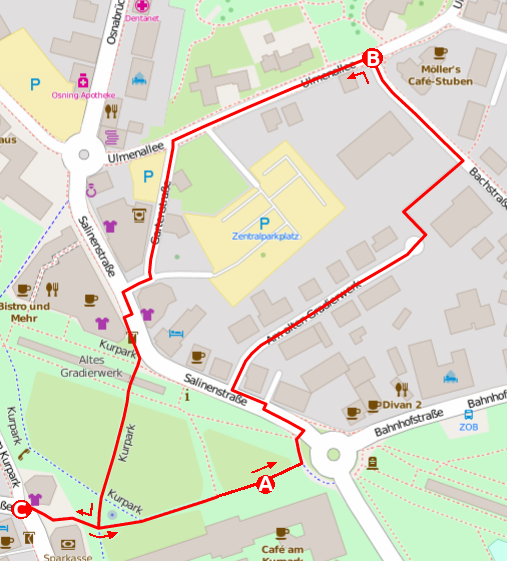
\includegraphics[width=\textwidth]{pics/png/01_Ergebnis_Small_Tour.png}
	\caption{Visualisierung der Route \textit{Bad Rothenfelde - Zentrum}. }
	\label{pic:small_tour}
	\end{center}
\end{figure}

Die städtische Umgebung, wodurch die Route $R$ verläuft, weißt keine Steigungen bzw. Gefälle größer als 5\% auf. Dennoch sind im errechneten, blauen Leistungsprofil in der Abbildung \ref{pic:power_small_tour} äußerst große Schwankungen zu entdecken. Es wurden nur drei verschiedene Laufgeschwindigkeiten gestellt (siehe \ref{pic:run_small_tour}: 5 km/h, 7.5 km/h und 11 km/h), entsprechend sieht das errechnete Leistungsprofil nur grob dem gewünschten Leistungsprofil (in gelb) ähnlich. Je mehr Geschwindigkeitsstufen $V_m$ gestellt werden, desto besser schmiegt sich das errechnete Leistungsprofil an das gewünschte Profil. 

\begin{figure}[ht]
	\begin{center}
	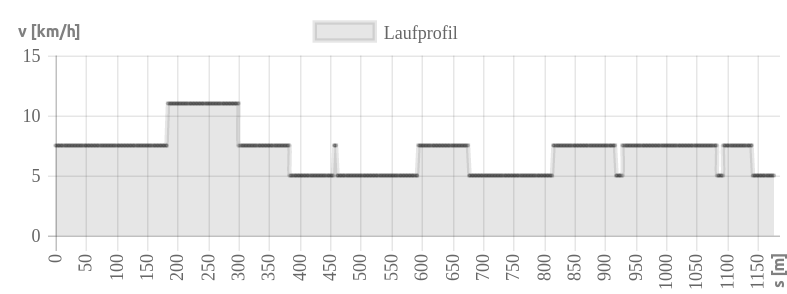
\includegraphics[width=\textwidth]{pics/png/03_Laufprofil_Small_Tour.png}
	\caption{Laufprofil vom Beispiel \textit{Bad Rothenfelde Zentrum}}
	\label{pic:run_small_tour}
	\end{center}
\end{figure}

\begin{figure}[ht]
	\begin{center}
	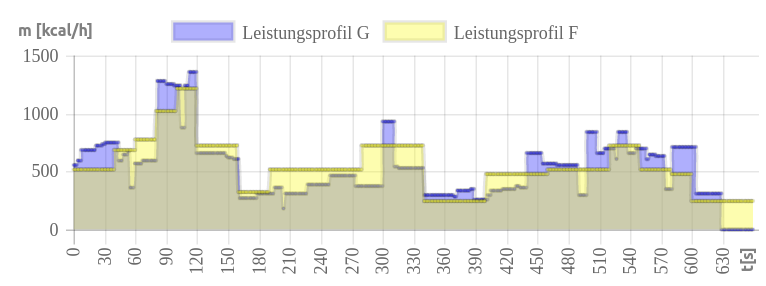
\includegraphics[width=\textwidth]{pics/png/05_Leistungsprofil_Small_Tour.png}
	\caption{Leistungsprofil vom Beispiel \textit{Bad Rothenfelde Zentrum} (blau) im Vergleich zum geforderten Leistungsprofil (gelb)}
	\label{pic:power_small_tour}
	\end{center}
\end{figure}

\pagebreak

In einer weiteren Rundtour (siehe Abbildung \ref{pic:big_tour}) ist eine weitaus größere Tour durch den gebirgigen Teutoburgerwald generiert worden. Auf der Route existierenden Gefälle von bis zu 30\%; Entsprechend konnten für einige Etappen nur negative Energiewerte berechnet werden bei maximaler Laufgeschwindigkeit. Solche Berechnungen wären aufgrund der - für diese Umstände - ungeeignete Energieformel fatal und für eine vernünftige Anwendung inakzeptabel.

\section{Fazit und Ausblick}\label{fazit}
In dieser Arbeit wird eine Möglichkeit aufgezeigt, wie man strecken-abhängige Laufprofile auf zeit-abhängige Leistungsprofile optimieren kann. Es existieren jedoch noch einige Aspekte, weshalb die vorgestellten Möglichkeiten noch nicht vollständig anwendbar sind: Dabei handelt es sich um die Genauigkeit des Modells, die rudimentäre Rundtour-Generierung und einer Echtzeit-Anpassung. Eine minimale Verfälschung des zeitabhängigen Profils wird aufgrund der konstanten Etappen im Modell immer vorhanden sein. Die Genauigkeit des vorgestellten Modells lässt sich nur schwer optimieren. Durch die eher veraltete Energieformel und den relativ grob aufgelösten Höhendatensatz sind Ungenauigkeiten gegeben. Die dargestellten Ergebnisse vom Optimierungsalgorithmus hingegen sind zufriedenstellend. Die automatische Generierung der Rundtour kann in Zukunft noch weiter optimiert werden. Es ist sehr wahrscheinlich, dass es Alternativrouten gibt, die das gewünschte Leistungsprofil aufgrund ihrer terrestrischen Eigenschaften besser annähern, als die primär gestellte Route. Eine lokale Suche für alternative Routen wäre denkbar, indem einzelne Stützpunkte versetzt werden. Vorstellbar wären, nicht nur Graphen aus einem Liniensegment optimiert werden, sondern auch komplexere, azyklische Graphen mit Verzweigungen. Die Erstellung eines solchen Graphen könnte z.B. durch zufällig- vorgegebene Linienbänder erfolgen, wie es in Abbildung \ref{pic:ring_schaplone} visualisiert ist. Selbst bei optimal geplanten Routen wird man wahrscheinlich nie alle anthropogenen Einflüsse in das Modell mit einbeziehen können. Die Anwendung muss sich letztlich für das Monitoring auf die Messwerte verlassen muss, die während des Durchlaufs der Tour gemessen werden. Diese Daten können dann verwendet werden, um gegebenenfalls während des Routenverlaufes die restliche Tour anzupassen - beispielsweise durch eine Verkürzung der Gesamtstrecke, falls der Patient die gewünschte Leistung nicht aufbringen kann. Abweichungen werden vom Monitoring erkannt und in Echtzeit umgesetzt. Dies kann vorkommen, wenn der Patient durch natürliche und temporäre Barrieren auf seiner Tour aufgehalten wird oder eigenwillig sogar die Strecke vorübergehend verlässt. \\
Der in dieser Arbeit erschaffene Algorithmus bietet die Grundlage für eine zuverlässige, gesundheitsfördernde Anwendung. Wenn an all den genannten Aspekten weiter gearbeitet wird, könnte diese Anwendung in Zukunft auch den Menschen zur Verfügung gestellt werden. 

\begin{figure}[ht]
	\begin{center}
	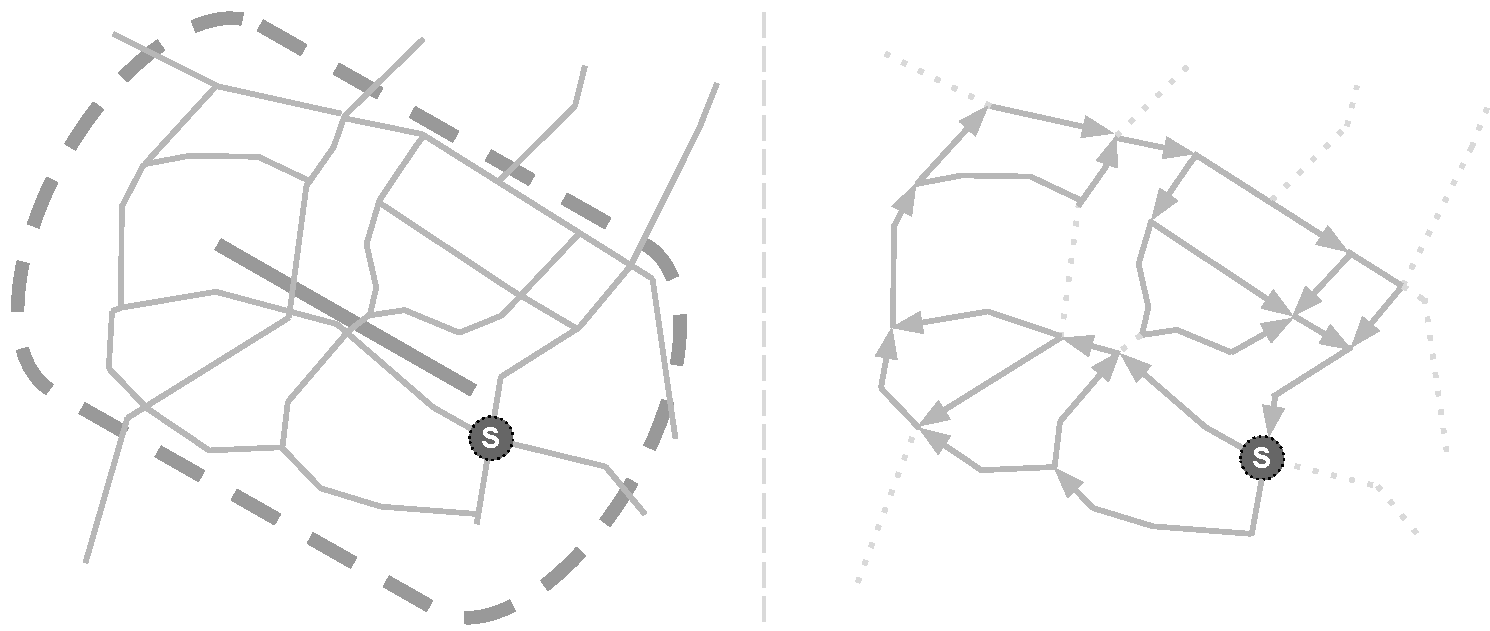
\includegraphics[width=\textwidth]{pics/pdf/011_Ring_Schaplone.pdf}
	\caption{Vorstellung, wie man einen azyklischen Graphen aus einem Linienband bzw. Ring einen azyklischen Graphen extrahieren kann, um daraus eine Joggingroute zu erstellen.}
	\label{pic:ring_schaplone}
	\end{center}
\end{figure}

\pagebreak

\addcontentsline{toc}{section}{Literatur}

\bibliography{Literatur}

\addcontentsline{toc}{section}{Abbildungsverzeichnis}

\pagebreak

\listoffigures

\pagebreak

\addcontentsline{toc}{section}{Anlagen}

\begin{figure}[hp]
	\begin{center}
	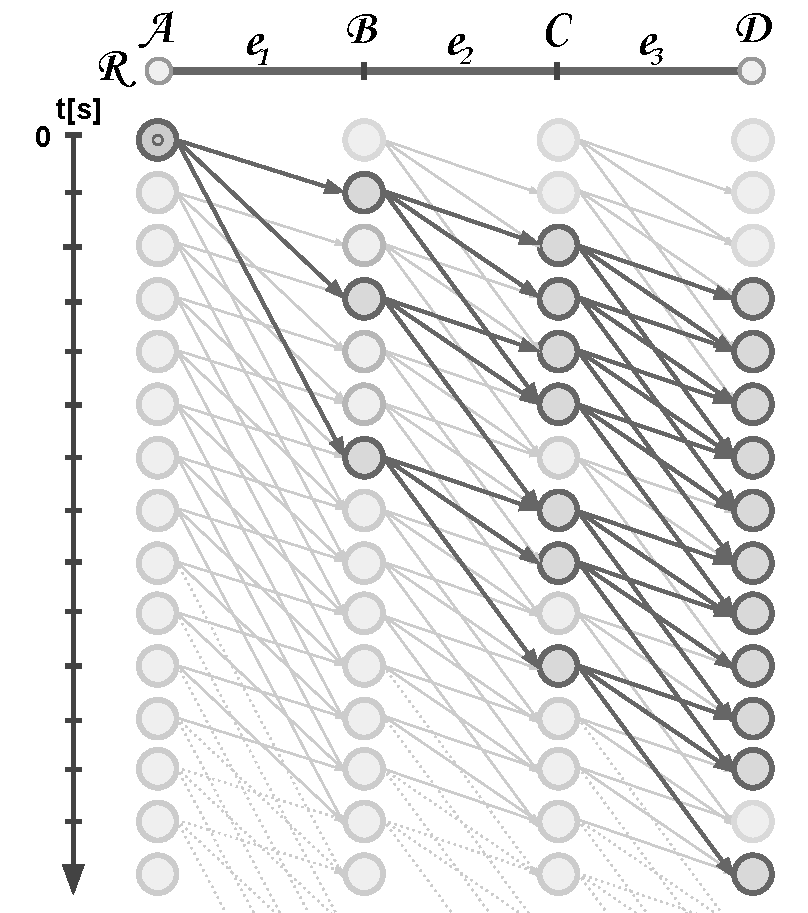
\includegraphics[width=\textwidth]{pics/pdf/006_Graph_der_Optimierung_Richtig.pdf}
	\caption{Komplexere Graphvorstellung - ausgehende Kanten eines Meilensteins transistieren zum nächsten Meilenstein zu verschiedenen Zeitpunkten }
	\label{pic:graph_right}
	\end{center}
\end{figure}

\begin{figure}[hp]
	\begin{center}
	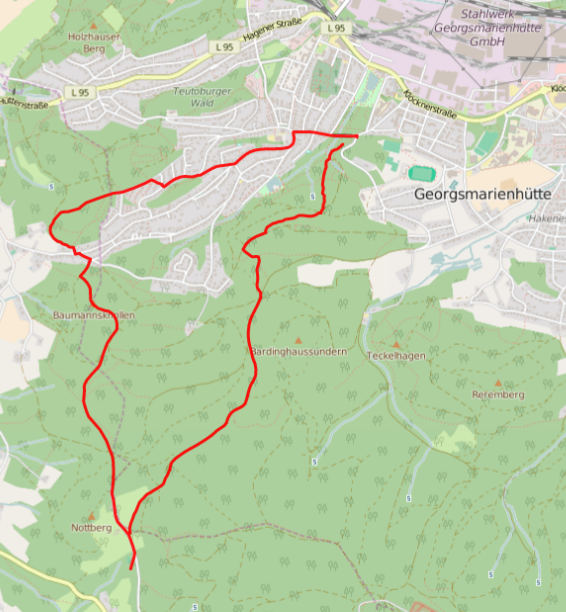
\includegraphics[width=\textwidth]{pics/png/02_Ergebnis_Big_Huette.png}
	\caption{Verlauf der Route \textit{Alt-Georgsmarienhütte}. Gesamtlänge 7950 Meter.}
	\label{pic:big_tour}
	\end{center}
\end{figure}

\end{document}
